\documentclass{beamer}

\usefonttheme{professionalfonts} % using non standard fonts for beamer
\usefonttheme{serif} % default family is serif

\usepackage{enumitem}
\setitemize{label=\usebeamerfont*{itemize item}%
  \usebeamercolor[fg]{itemize item}
  \usebeamertemplate{itemize item}}

\usepackage{hyperref}
\usepackage{booktabs}
\usepackage{xfp}
\usepackage{graphicx}
\def\Put(#1,#2)#3{\leavevmode\makebox(0,0){\put(#1,#2){#3}}}
\usepackage{colortbl}
\usepackage{tikz}
\usepackage{amssymb}
\usepackage{enumerate}
\usepackage{arydshln}
\usepackage{algorithm}
\usepackage{algpseudocode}
\usepackage{subcaption} %to have subfigures available

\usepackage[absolute,overlay]{textpos}

\colorlet{lightred}{red!25}
\colorlet{lightgreen}{green!25}
\beamertemplatenavigationsymbolsempty

\newcommand\blfootnote[1]{%
  \begingroup
  \renewcommand\thefootnote{}\footnote{#1}%
  \addtocounter{footnote}{-1}%
  \endgroup
}

\makeatletter

%% Textclass specific LaTeX commands.
\newcommand\makebeamertitle{\frame{\maketitle}}%
\AtBeginDocument{%
  \let\origtableofcontents=\tableofcontents
  \def\tableofcontents{\@ifnextchar[{\origtableofcontents}{\gobbletableofcontents}}
  \def\gobbletableofcontents#1{\origtableofcontents}
}
%% User specified LaTeX commands.
\usetheme{Malmoe}
\useoutertheme{infolines}
\addtobeamertemplate{headline}{}{\vskip2pt}
\setbeamercovered{transparent}

\title[PFlock report]{PFLOCK Report}
\author[AC]{Andres Calderon}
\institute[UCR]{University of California, Riverside}
\makeatother

%%%%%%%%%%%%%%%%%%%%%%%%%%%%%%%%%%%%%%
%% Main document
%%%%%%%%%%%%%%%%%%%%%%%%%%%%%%%%%%%%%%
\begin{document}
\makebeamertitle
\newif\iflattersubsect

\AtBeginSection[] {
    \begin{frame}<beamer>
    \frametitle{Outline} 
    \tableofcontents[currentsection]  
    \end{frame}
    \lattersubsectfalse
}

\AtBeginSubsection[] {
    \begin{frame}<beamer>
    \frametitle{Outline} 
    \tableofcontents[currentsubsection]  
    \end{frame}
}

%%%%%%%%%%%%%%%%%%%%%%%%%%%%%%%%%%%%%%%%%%%
%%% Slides...
%%%%%%%%%%%%%%%%%%%%%%%%%%%%%%%%%%%%%%%%%%%

\begin{frame}{Issues with eBird dataset...}
    \begin{itemize}
        \item For California:
        \begin{itemize}
            \item Number of observations: 59'807.295
            \item Number of unique spatio-temporal observations: 3'098.425
            \item Number of unique spatial observations: 450.434
        \end{itemize}
        \item Grouped by time:
        \begin{itemize}
            \item per hour: More crowed intervals $\longrightarrow$ 2916, 2871, 2839.
            \item per day : More crowed intervals $\longrightarrow$ 2966, 2901, 2886.
        \end{itemize}
        \item Grouped by Entity Id: all distinct! The Id is the observation Id not the observer Id =(
    \end{itemize}
\end{frame}

\begin{frame}{Checking C++ BFE and PSI implementation...}
    \begin{itemize}
        \item Using a relatively small dataset:
        \begin{itemize}
            \item Berlin dataset
            \item Created using Brinkhoff\footnote{\url{https://iapg.jade-hs.de/en/members/brinkhoff/generator}} Trajectory Generator
            \item ~20K points per time instant, 10 consecutive time instants...
        \end{itemize}
    \end{itemize}
\end{frame}

\begin{frame}{Checking C++ BFE and PSI implementation using Berlin dataset...}
    \centering
    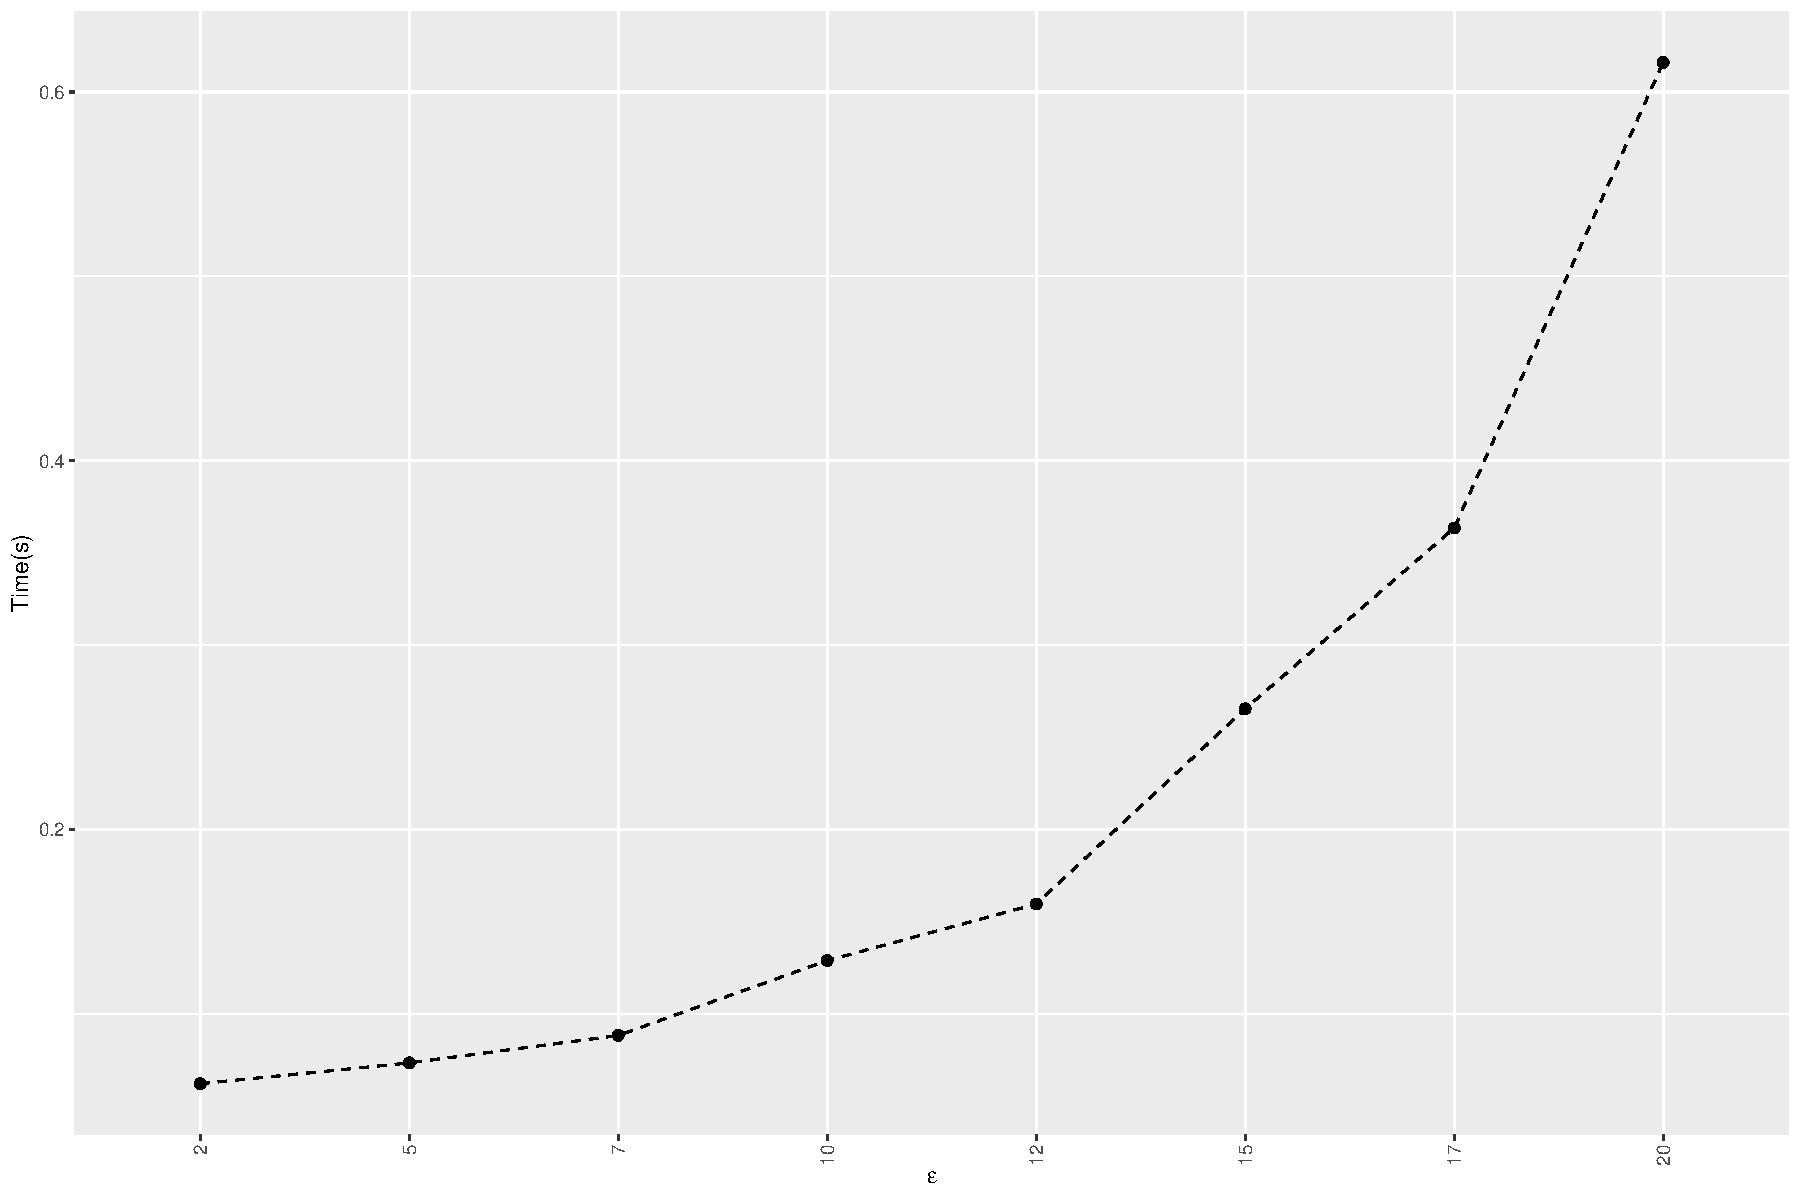
\includegraphics[width=0.8\textwidth]{scripts/epsilon_benchmark}
\end{frame}
\begin{frame}{Checking C++ BFE and PSI implementation using Berlin dataset...}
    \centering
    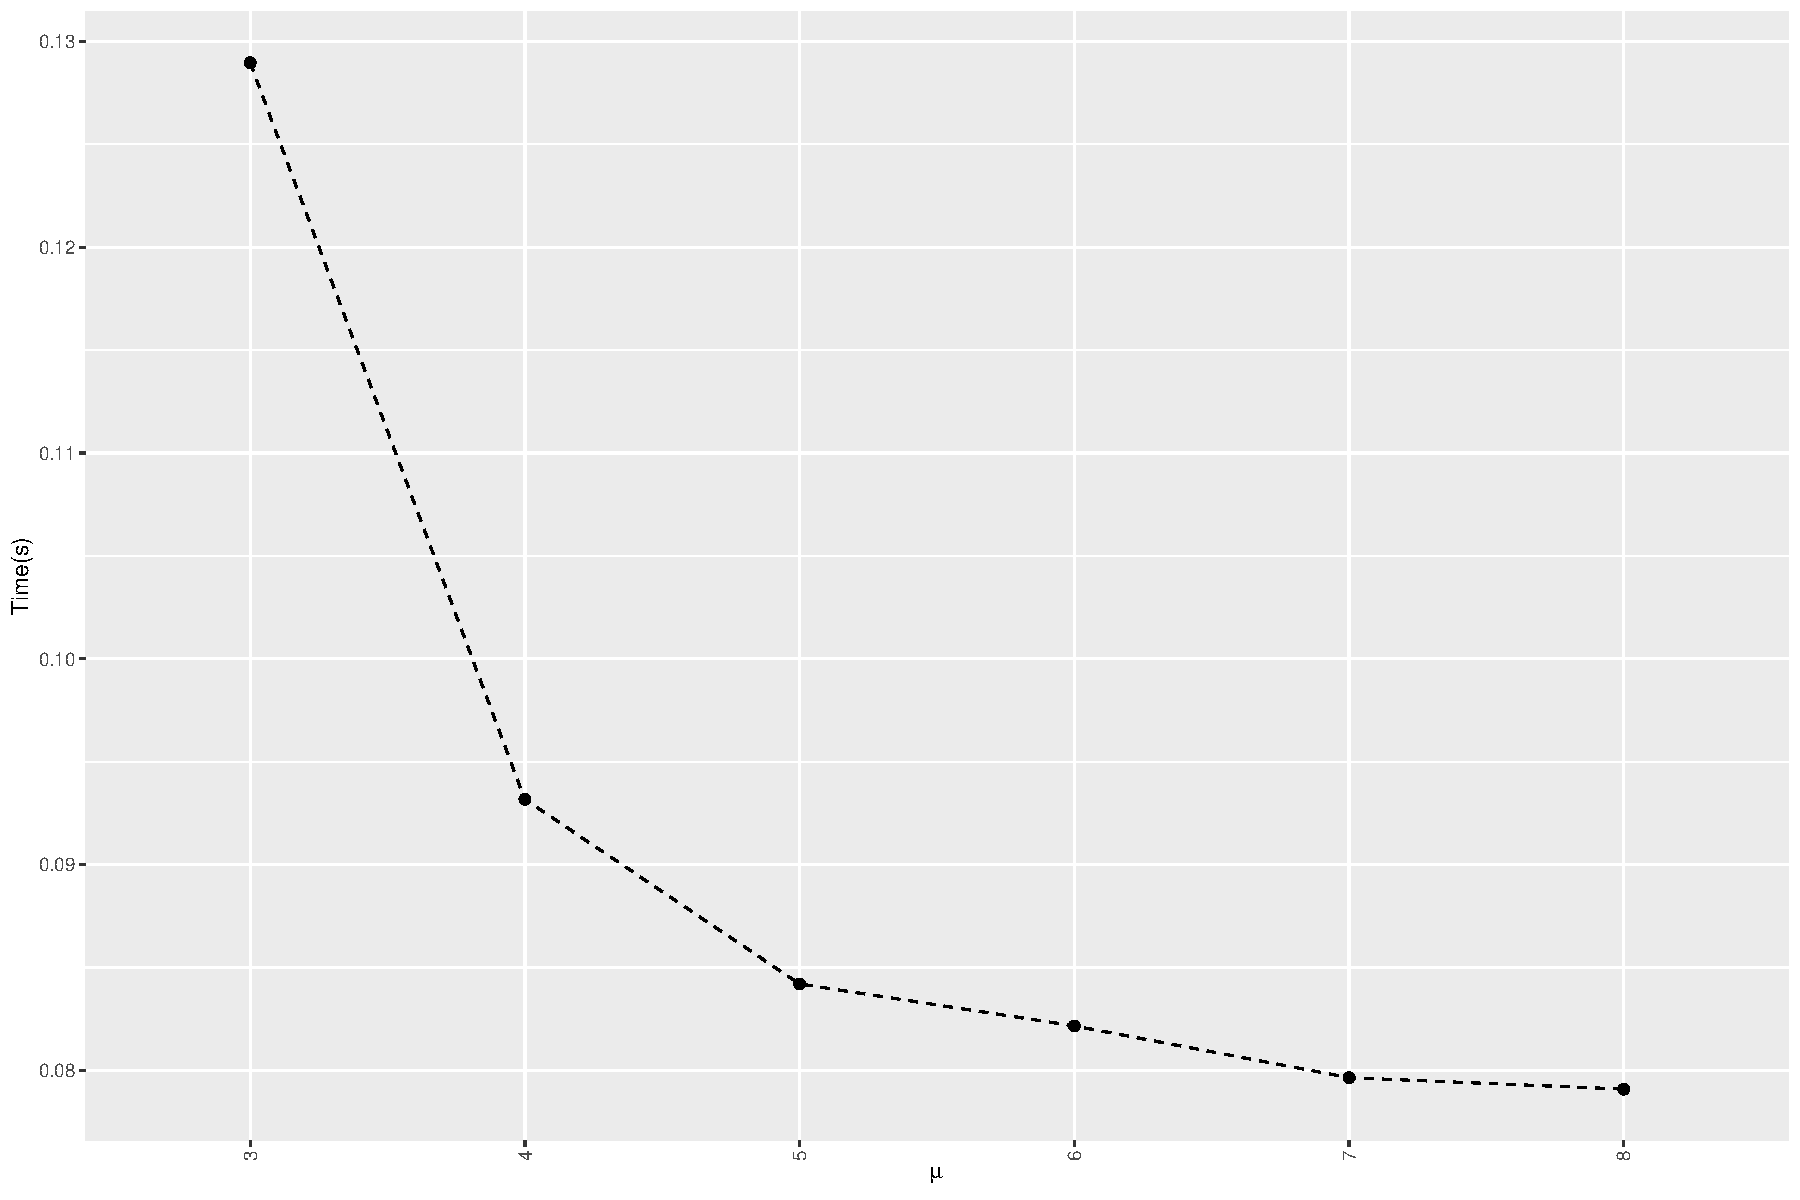
\includegraphics[width=0.8\textwidth]{scripts/mu_benchmark}
\end{frame}
\begin{frame}{Checking C++ BFE and PSI implementation using Berlin dataset...}
    \centering
    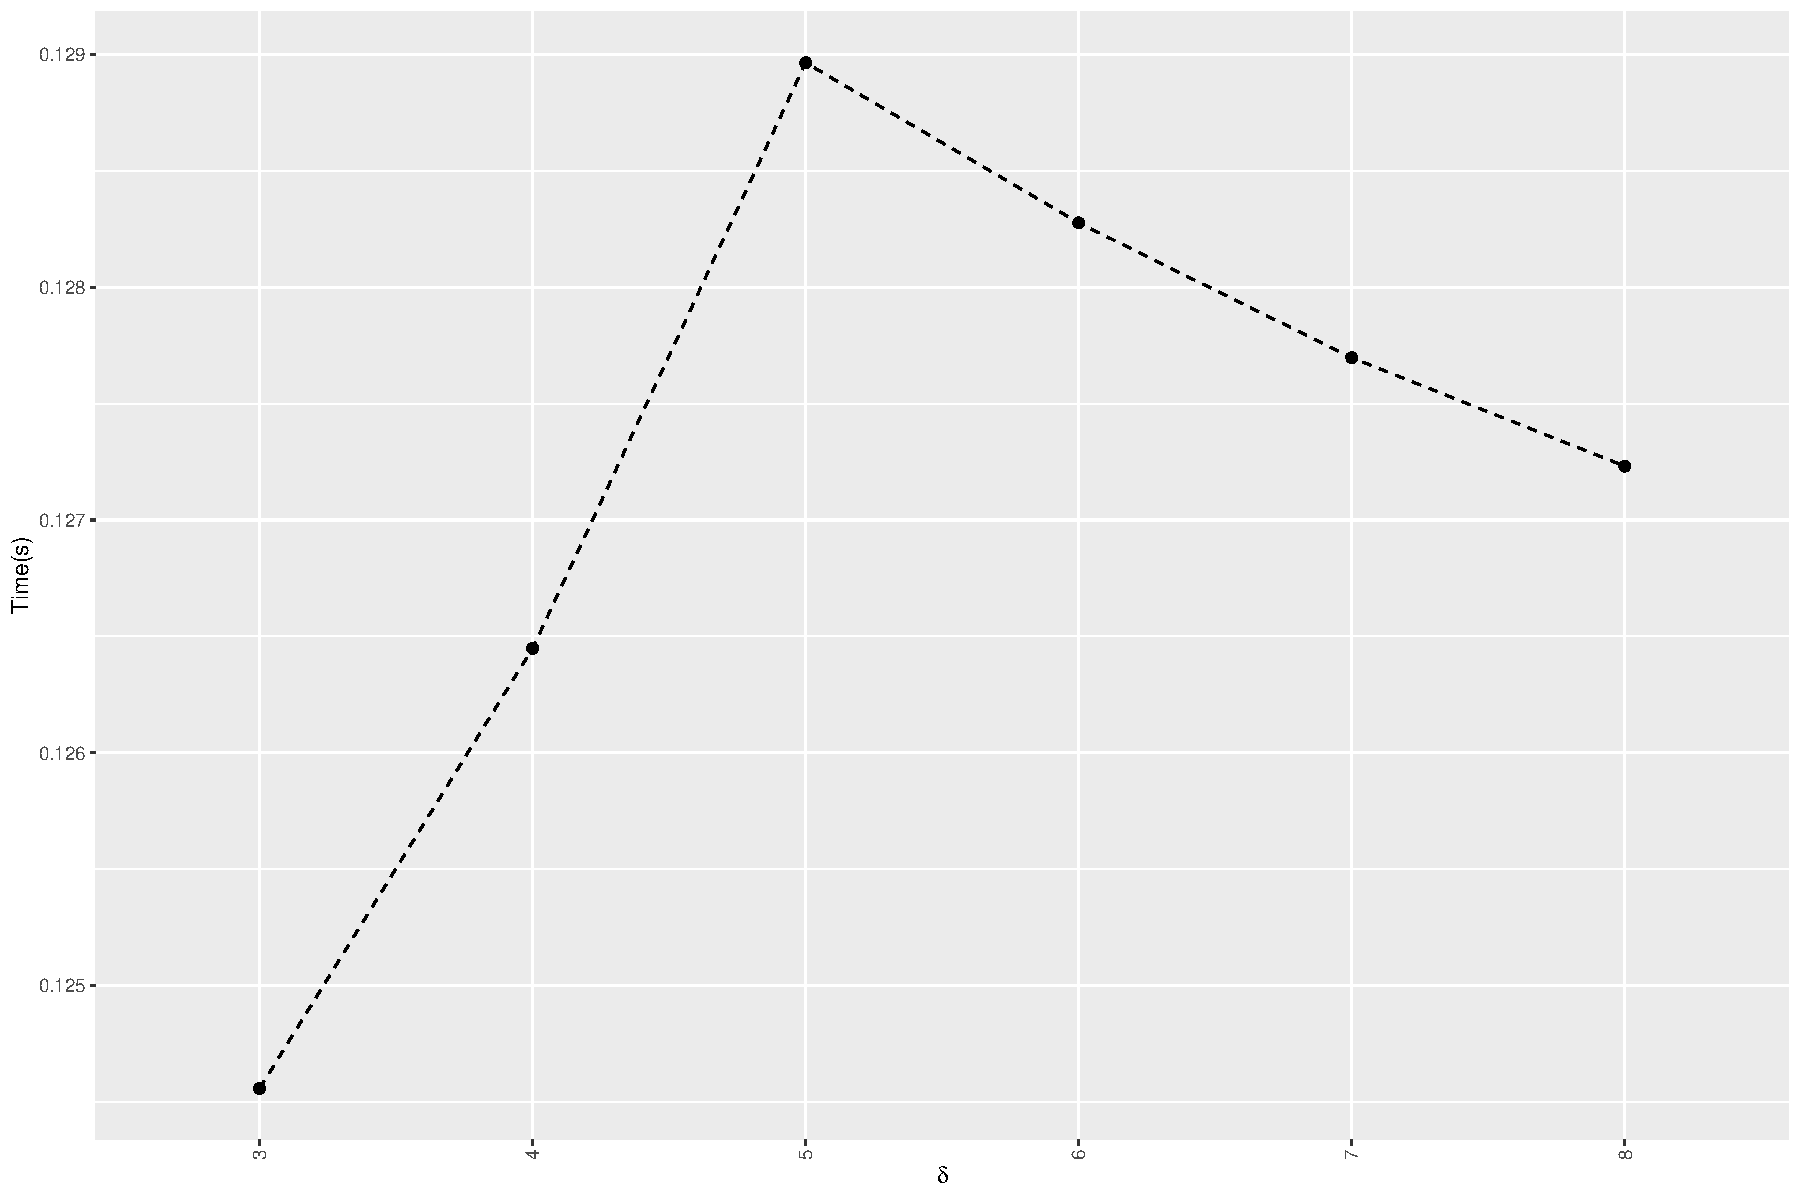
\includegraphics[width=0.8\textwidth]{scripts/delta_benchmark}
\end{frame}


\begin{frame}{What is next?...}
    \begin{itemize}
        \item Scala implementation of BFE was updated and is already done.
        \item Currently working on Scala implementation of the Inverted Index proposal in PSI...
        \item Expecting run tests using Berlin dataset and compare with C++ implementation...
        \item Then running performance experiments over L.A. dataset...
    \end{itemize}
\end{frame}

%%%%%%%%%%%%%%%%%%%%%%%%%%%%%%%%%%%%%%%%%%%

\end{document}

